\documentclass[12pt, oneside]{article}   	
\usepackage{geometry}                		
\geometry{letterpaper}                   		

\usepackage{graphicx}				
								
\usepackage{amssymb}
\usepackage[T1]{fontenc}
\usepackage{lmodern}
\usepackage{fixltx2e}
\usepackage{mathtools}
\usepackage{enumerate}
\usepackage{floatrow}
\usepackage{listings}

\usepackage{color}

\definecolor{mygreen}{rgb}{0,0.6,0}
\definecolor{mygray}{rgb}{0.5,0.5,0.5}
\definecolor{mymauve}{rgb}{0.58,0,0.82}

\lstset{ 
  basicstyle=\footnotesize,        
  breakatwhitespace=false,         
  breaklines=true,                 
  deletekeywords={YEAR},            
  keepspaces=true,                 
  keywordstyle=\color{blue},       
  stringstyle=\color{mymauve},     
}

\newcommand{\itab}[1]{\hspace{0em}\rlap{#1}}
\newcommand{\tab}[1]{\hspace{.2\textwidth}\rlap{#1}}

\title{Selected Exercises from Fundamentals of Database Systems}
\author{Andrew Kowalczyk}
\date{}

\begin{document}

\maketitle
I selected around 40 questions from the 6$^{th}$ edition of \textit{Fundamentals of Database Systems} by Ramez Elmasri and Shamkant Navathe. This was part of my requirement for my Introduction to Database Systems course taken in the Fall of 2013.

\pagebreak
\tableofcontents
\pagebreak

\section*{Chapter 1}
\addcontentsline{toc}{section}{Chapter 1}

\subsection*{1.8 Identify some informal queries and update operations that you would expect to apply to the database shown in Figure 1.2.}
\addcontentsline{toc}{subsection}{1.8}

\subsubsection*{Queries}

\begin{enumerate}
\item What are the prerequisites of the Database course?
\item Find the names of all students majoring in Mathematics.
\item Find the the transcript of the student named Brown.
\end{enumerate}

\subsubsection*{Updates}

\begin{enumerate}
\item Insert a new student in the database whose Name=Kowalczyk, Student\_number=25, Class=4, and Major=CS.
\item Change the grade that Brown received in Discrete Mathematics to a D.
\end{enumerate}

\subsection*{1.9 What is the difference between controlled and uncontrolled redundancy? Illustrate with examples.}
\addcontentsline{toc}{subsection}{1.9}
Redundancy is the term given when the same data is stored multiple times in several places in a database. If you look at Figure 1.5(a)  in the text, you can see that the name of the student with Student\_number=8 is Brown is stored multiple times. Redundancy is controlled when the database management system (DBMS) ensures that multiple copies of the same data are consistent. To illustrate this, let's say we are adding a new record with Student\_number=8 to be stored in the database of Figure 1.5(a). If we were to have uncontrolled redundancy, the DBMS would have no control over this. If we were to have controlled redundancy, the DBMS would ensure that Student\_name=Brown in that record.

\subsection*{1.10 Specify all the relationships among the records of the database shown in Figure 1.2.}
\addcontentsline{toc}{subsection}{1.10}
\begin{enumerate}
\item Every GRADE\_REPORT record is related to one STUDENT record and one SECTION record.
\item Every SECTION record is related to a COURSE record.
\item Every PREREQUISITE record relates two COURSE records. One being a course and the other being a prerequisite to that course.
\end{enumerate}

\subsection*{1.11 Give some additional views that may be needed by other user groups for the database shown in Figure 1.2.}
\addcontentsline{toc}{subsection}{1.11}
\begin{enumerate}
\item A view of each class section that groups all the students who took that section and their respective grade.
\item A view that gives the number of courses taken and the grade point average for each student.
\end{enumerate}

\subsection*{1.12 Cite some examples of integrity constraints that you think can apply to the database shown in Figure 1.2.}
\addcontentsline{toc}{subsection}{1.12}
\subsubsection*{Key constraints}
\begin{enumerate}
\item Student\_number must be unique for each STUDENT record.
\item Course\_number must be unique for each COURSE record.
\end{enumerate}

\subsubsection*{Referential integrity constraints}
\begin{enumerate}
\item The Course\_number in a SECTION record must also exist in some COURSE record.
\item The Student\_number in a GRADE\_REPORT record must also exist in some STUDENT record.
\end{enumerate}

\subsubsection*{Domain constraints}
\begin{enumerate}
\item Grades in a a given GRADE\_REPORT record must be one of these values: {A, B, C, D, F, I, W}.
\end{enumerate}
\section*{Chapter 2}
\subsection*{2.12 Think of different users for the database shown in Figure 1.2. What types of applications would each user need? To which user category would each belong, and what type of interface would each need?}

\begin{enumerate}
  \item Students add and drop classes. Actions that they can do are as listed:
    \begin{enumerate}
       \item Register themselves in a section of a course
       \item Drop themselves from a section of a course 
    \end{enumerate}
  \item Registrar. They enter data of registration of students in sections of courses, and later enter the grades of the students. Actions that they can do are as listed:
    \begin{enumerate}
        \item Check whether a student who is registered in a course has the appropriate prerequisite courses
       \item Add a student to a section of a course
       \item Enter the student grades for a section
    \end{enumerate}
  \item Admissions. Their main application would be to enter newly accepted students into the database. Actions that they can do are as listed:
    \begin{enumerate}
    	\item Add students to the school's records
    \end{enumerate}
\end{enumerate}
\section*{Chapter 3}
\subsection*{3.11 Suppose that each of the following Update operations is applied directly to the database state shown in Figure 3.6. Discuss all integrity constraints violated by each operation, if any, and the different ways of enforcing these constraints.}

In each of examples, the different ways of enforcing the constraints is listed in preferential order (\textit{i.e.} 1 is most preferred, 2 is less preferred, etc.).

\subsubsection*{(a) Insert <"Robert", "F", "Scott", "943775543", "1972-06-21", "2365 Newcastle Rd, Bellaire, TX", M, 58000, "888665555", 1> into EMPLOYEE.}
No constraints violated.

\subsubsection*{(b) Insert <"ProductA", 4, "Bellaire", 2> into PROJECT.}
 Since there is no tuple in the DEPARTMENT relation with DNUM=2, this insertion would violate referential integrity for that very reason. We can enforce the constraint with these options:
\begin{enumerate}
\item Rejecting the insertion
\item Changing the value of DNUM in the new PROJECT tuple to an existing DNUMBER value in the DEPARTMENT relation
\item Inserting a new DEPARTMENT tuple with DNUMBER=2
\end{enumerate}

\subsubsection*{(c) Insert <"Production", 4, "943775543", "2007-10-01"> into DEPARTMENT.}
Oh no! Since there already exists a DEPARTMENT tuple with DNUMBER=4, this would violate the key constraint. Enforcement of this constraint would happen by:
\begin{enumerate}
\item Rejecting the insertion
\item Changing the value of DNUMBER in the new DEPARTMENT tuple to a value that does not violate the key constraint
\end{enumerate}
Also, since there is no tuple in the EMPLOYEE relation with SSN="943775543", this insertion also happens to violate referential integrity. Let us enforce the constraint by either: 
\begin{enumerate}
\item Rejecting the insertion
\item Changing the value of MGRSSN to an existing SSN value in EMPLOYEE
\item Inserting a new EMPLOYEE tuple with SSN="943775543"
\end{enumerate}

\subsubsection*{(d) Insert <"677678989", NULL, "40.0"> into WORKS\_ON.}
Since PNO (part of the primary key of WORKS\_ON) is null, this violates entity integrity. We have these options to enforce this constraint:
\begin{enumerate}
\item Rejecting the insertion
\item Changing the value of PNO in the new WORKS\_ON tuple to a value of PNUMBER that exists in the PROJECT relation
\end{enumerate}
Since there is no tuple in the EMPLOYEE relation with SSN="677678989", this insertion would violate referential integrity. We may enforce the constraint by:
\begin{enumerate}
\item Rejecting the insertion
\item Changing the value of ESSN to an existing SSN value in EMPLOYEE
\item Inserting a new EMPLOYEE tuple with SSN="677678989"
\end{enumerate}

\subsubsection*{(e) Insert <"453453453","John","M","1990-12-12","spouse"> into DEPENDENT.}
Nope! Not a single constraint was violated.

\subsubsection*{(f) Delete the WORKS\_ON tuples with Essn = "333445555".}
No constraints violated in the making of this delete.

\subsubsection*{(g) Delete the EMPLOYEE tuple with Ssn = "987654321".}
Unfortunately, the employee trying to be deleted is referenced in the WORKS\_ON, DEPENDENT, DEPARTMENT, and EMPLOYEE relations. We can enforce such an abolishment by either:
\begin{enumerate}
\item Rejecting the deletion
\item Deleting all tuples in the WORKS\_ON, DEPENDENT, DEPARTMENT, and EMPLOYEE relations whose values for ESSN, ESSN, MGRSSN, and SUPERSSN, respectively, is equal to "987654321"
\end{enumerate}

\subsubsection*{(h) Delete the PROJECT tuple with Pname="ProductX".}
This deletion would completely violate referential integrity because two tuples exist in the WORKS\_ON relation that reference the tuple being deleted from PROJECT. Silly us,  let's enforce the constraint by:
\begin{enumerate} 
\item Rejecting the deletion
\item Deleting the tuples in the WORKS\_ON relation whose value for the primary key PNUMBER for the tuple being deleted from PROJECT with PNO=1
\end{enumerate}

\subsubsection*{(i) Modify the Mgr\_ssn and Mgr\_start\_date of the DEPARTMENT tuple with Dnumber = 5 to "123456789" and "2007-10-01", respectively.}
No violation of constraints.

\subsubsection*{(j) Modify the Super\_ssn attribute of the EMPLOYEE tuple with Ssn = "999887777" to "943775543".}
Goodness gracious, great balls of fire! Since there is no tuple in the EMPLOYEE relation with SSN="943775543", this update would violate referential integrity. In order to enforce this constraint, we can choose from:
\begin{enumerate}
\item Rejecting the deletion
\item Inserting a new EMPLOYEE tuple with SSN="943775543"
\end{enumerate}

\subsubsection*{(k) Modify the Hours attribute of the WORKS\_ON tuple with Essn = "999887777" and Pno = 10 to "5.0".}
No constraints violated.
\section*{Chapter 4}
\addcontentsline{toc}{section}{Chapter 4}

\subsection*{4.9 How can the key and foreign key constraints be enforced by the DBMS? Is the enforcement technique you suggest difficult to implement? Can the constraint checks be executed efficiently when updates are applied to the database?}
\addcontentsline{toc}{subsection}{4.9}

In order to check efficiently for the key constraint, one can create an index on all of the attributes that form each primary or secondary key. Even before the new record is inserted, each index is searched to insure that no value currently exists in the index that matches the key value in the new record. If this is the case, the record is inserted successfully and we are happy.

In order to check efficiently for the foreign key constraint, the primary key is given an index for each referenced relation. Due to this, the check efficient enough for our purposes. Each time a new record is inserted in a referencing relation, we search the index for the primary key of the referenced relation. The value of its foreign key is used to accomplish this. The new record can be successfully inserted in the referencing relation if the referenced record exists. For the deletion of any given referenced record, an index on the foreign key of each of the referencing relations is very useful. We want to efficiently determine whether any records reference that given record. If the techniques described above do not exist, then, unfortunately, we must do linear searches to check for any of the above constraints. This would making the checks quite inefficient, and it would make us unhappy.


\subsection*{4.12 Specify the following queries in SQL on the database schema of Figure 1.2.}
\addcontentsline{toc}{subsection}{4.12}
\subsubsection*{(a) Retrieve the names of all senior students majoring in "CS" (computer sci- ence).}
\begin{lstlisting}[language=SQL]
SELECT Name 
FROM   STUDENT
WHERE  Major="CS"
    AND Class="4"
\end{lstlisting}

\subsubsection*{(b) Retrieve the names of all courses taught by Professor King in 2007 and 2008.}
\begin{lstlisting}[language=SQL]
SELECT Course_name
FROM   COURSE,
       SECTION
WHERE COURSE.Course_number=SECTION.Course_number
    AND Instructor="King"
    AND (Year="07" OR Year="08")
\end{lstlisting}

\subsubsection*{(c) For each section taught by Professor King, retrieve the course number, semester, year, and number of students who took the section.}
\begin{lstlisting}[language=SQL]
SELECT Course_number,
       Semester,
       Year,
       COUNT(*)
FROM   SECTION,
       GRADE_REPORT
WHERE Instructor="King"
    AND SECTION.Section_identifier=GRADE_REPORT.Section_identifier
GROUP BY Course_number, Semester, Year
\end{lstlisting}

\subsubsection*{(d) Retrieve the name and transcript of each senior student (Class = 4) majoring in CS. A transcript includes course name, course number, credit hours, semester, year, and grade for each course completed by the student.}
\begin{lstlisting}[language=SQL]
SELECT Name,
       C.Course_name,
       C.Course_number,
       Credit_hours,
       Semester,
       Year,
       Grade
FROM   STUDENT ST,
       COURSE C,
       SECTION S,
       GRADE_REPORT G
WHERE Class=4 
    AND Major="CS"
    AND ST.StudentNumber=G.StudentNumber
    AND G.Section_identifier=S.Section_identifier
    AND S.Course_number=C.Course_number
\end{lstlisting}
\section*{Chapter 6}

\subsection*{6.15. Show the result of each of the sample queries in Section 6.5 as it would apply to the database state in Figure 3.6.} 

\subsubsection*{Query 1: Find the name and address of all employees who work for the 'Research' department.}
\begin{center}
\begin{tabular}{ c | c | c }
  FNAME & LNAME & ADDRESS \\ \hline
  John & Smith & 731 Fondren, Houston, TX \\
  Franklin & Wong & 638 Voss, Houston, TX \\
  Ramesh &  Narayan & 975 Fire Oak, Humble, TX \\
  Joyce & English & 5631 Rice, Houston, TX \\
\end{tabular}
\end{center}

\subsubsection*{Query 2: For every project located in 'Stafford', list the project number, the controlling department number, and the department manager's last name, address, and birth date.}
\begin{center} 
\begin{tabular}{ c | c | c | c | c}
  PNUMBER & DNUM & LNAME & ADDRESS & BDATE \\ \hline
  10 & 4 & Wallace & 291 Berry, Bellaire, TX &20-JUN-31 \\
  30 & 4 & Wallace & 291 Berry, Bellaire, TX & 20-JUN-31 \\ 
\end{tabular}
\end{center}

\subsubsection*{Query 3: Find the names of all employees who work on all the projects controlled by department number 5.}
\begin{center}
\begin{tabular}{ c | c }
  LNAME & FNAME \\ \hline
\end{tabular}
\end{center}

\subsubsection*{Query 4: Make a list of project numbers for projects that involve an employee whose last name is 'Smith' as a worker or as a manager of the department that controls the project.}
\begin{center}
\begin{tabular}{ c }
  PNO \\ \hline
  1 \\
  2 \\
\end{tabular}
\end{center}

\subsubsection*{Query 5: List the names of all employees with two or more dependents.}
\begin{center}
\begin{tabular}{ c | c }
  LNAME & FNAME \\ \hline
  Smith & John \\
  Wong & Franklin \\
\end{tabular}
\end{center}

\subsubsection*{Query 6 List the names of employees who have no dependents.}
\begin{center}
\begin{tabular}{ c | c }
  LNAME & FNAME \\ \hline
  Zelaya & Alicia \\
  Narayan & Ramesh \\
  English & Joyce \\
  Jabbar & Ahmad \\
  Borg & James \\
\end{tabular}
\end{center}

\subsubsection*{Query 7: List the names of managers who have at least one dependent.}
\begin{center}
\begin{tabular}{ c | c }
  LNAME & FNAME \\ \hline
  Wallace & Jennifer \\
  Wong & Franklin \\
\end{tabular}
\end{center}

\subsection*{6.16 Specify the following queries on the COMPANY relational database schema shown in Figure 5.5, using the relational operators discussed in this chapter. Also show the result of each query as it would apply to the database state in Figure 3.6.}
I use the symbol $\sigma$ for SELECT, $\pi$ for PROJECT, $\rhd\lhd$ for EQUIJOIN, * for NATURAL JOIN, and $\mathfrak{F}$ for FUNCTION.

\subsubsection*{(a) Retrieve the names of employees in department 5 who work more than 10 hours per week on the "ProductX" project.}
\subsubsection*{Relational Operators}
EMP\_W\_X $\Leftarrow$ ( $\sigma$ \textsubscript{PNAME="ProductX"} (PROJECT)) $\rhd\lhd$ \textsubscript{(PNUMBER),(PNO)} (WORKS\_ON) \\
EMP\_WORK\_10 $\Leftarrow$ (EMPLOYEE) $\rhd\lhd$ \textsubscript{(SSN),(ESSN)} ( $\sigma$ \textsubscript{HOURS>10} (EMP\_W\_X)) \\
RESULT $\Leftarrow$ $\pi$ \textsubscript{LNAME,FNAME} ( $\sigma$ \textsubscript{DNO=5} (EMP\_WORK\_10))

\subsubsection*{Result}
\begin{center}
\begin{tabular}{ c | c }
  LNAME & FNAME \\ \hline
  Smith & John \\
  English & Joyce \\
\end{tabular}
\end{center}

\subsubsection*{(b) List the names of employees who have a dependent with the same first name as themselves.}
\subsubsection*{Relational Operators}
E $\Leftarrow$ (EMPLOYEE) $\rhd\lhd$ \textsubscript{(SSN,FNAME),(ESSN,DEPENDENT\_NAME)} (DEPENDENT)\\
R $\Leftarrow$ $\pi$ \textsubscript{LNAME,FNAME} (E)

\subsubsection*{Result}
\begin{center}
\begin{tabular}{ c | c }
  LNAME & FNAME \\ \hline
\end{tabular}
\end{center}

\subsubsection*{(c) Find the names of employees that are directly supervised by "Franklin Wong".}
\subsubsection*{Relational Operators}
WONG\_SSN $\Leftarrow$ $\pi$ \textsubscript{SSN} ( $\sigma$ \textsubscript{FNAME="Franklin" AND LNAME="Wong"} (EMPLOYEE))\\
WONG\_EMPS $\Leftarrow$ (EMPLOYEE) $\rhd\lhd$ \textsubscript{(SUPERSSN),(SSN)} (WONG\_SSN)\\
RESULT $\Leftarrow$ $\pi$ \textsubscript{LNAME,FNAME} (WONG\_EMPS)

\subsubsection*{Result}
\begin{center}
\begin{tabular}{ c | c }
  LNAME & FNAME \\ \hline
  Smith & John \\
  Narayan & Ramesh \\
  English & Joyce \\
\end{tabular}
\end{center}

\subsubsection*{(d) For each project, list the project name and the total hours per week (by all employees) spent on that project.}
\subsubsection*{Relational Operators}
PROJ\_HOURS(PNO,TOT\_HRS) $\Leftarrow$ \textsubscript{PNO} $\mathfrak{F}$ \textsubscript{SUM HOURS} (WORKS\_ON) \\
RESULT $\Leftarrow$ $\pi$ \textsubscript{PNAME,TOT\_HRS} ( (PROJ\_HOURS) $\rhd\lhd$ \textsubscript{(PNO),(PNUMBER)} (PROJECT) )

\subsubsection*{Result}  
\begin{center}
\begin{tabular}{ c | c }
  PNAME & TOT\_HRS  \\ \hline
  ProductX & 52.5 \\
  ProductY & 37.5 \\
  ProductZ & 50.0 \\
  Computerization & 55.0 \\
  Reorganization & 25.0 \\
  Newbenefits & 55.0 \\
\end{tabular}
\end{center}

\subsubsection*{(e) Retrieve the names of employees who work on every project.}
\subsubsection*{Relational Operators}
PROJ\_EMPS(PNO,SSN) $\Leftarrow$ $\pi$ \textsubscript{PNO,ESSN} (WORKS\_ON) \\
ALL\_PROJS(PNO) $\Leftarrow$ $\pi$ \textsubscript{PNUMBER} (PROJECT) \\
EMPS\_ALL\_PROJS $\Leftarrow$ PROJ\_EMPS $\div$ ALLPROJS \\
RESULT $\Leftarrow$ $\pi$ \textsubscript{LNAME,FNAME} (EMPLOYEE * EMP\_ALL\_PROJS)

\subsubsection*{Result}
\begin{center}
\begin{tabular}{ c | c }
  LNAME & FNAME \\ \hline
\end{tabular}
\end{center}

\subsubsection*{(f) Retrieve the names of employees who do not work on any project.}
\subsubsection*{Relational Operators}
ALL\_EMPS $\Leftarrow$ $\pi$ \textsubscript{SSN} (EMPLOYEE) \\
WORKING\_EMPS(SSN) $\Leftarrow$ $\pi$ \textsubscript{ESSN} (WORKS\_ON)\\
NON\_WORKING\_EMPS $\Leftarrow$ ALL\_EMPS - WORKING\_EMPS\\
RESULT $\Leftarrow$ $\pi$ \textsubscript{LNAME,FNAME} (EMPLOYEE * NON\_WORKING\_EMPS)

\subsubsection*{Result}
\begin{center}
\begin{tabular}{ c | c }
  LNAME & FNAME \\ \hline
\end{tabular}
\end{center}
\subsubsection*{(g) For each department, retrieve the department name and the average salary of all employees working in that department.}
\subsubsection*{Relational Operators}
DEPT\_AVG\_SALS(DNUMBER,AVG\_SAL) $\Leftarrow$ \textsubscript{DNO} $\mathfrak{F}$ \textsubscript{AVG SALARY} (EMPLOYEE)\\
RESULT $\Leftarrow$ $\pi$ \textsubscript{DNUMBER,AVG\_SAL} ( DEPT\_AVG\_SALS * DEPARTMENT )

\subsubsection*{Result}
\begin{center}
\begin{tabular}{ c | c }
  DNUMBER & AVG\_SAL  \\ \hline
  Research & 33250 \\
  Administration & 31000 \\
  Headquarters & 55000 \\
\end{tabular}
\end{center}

\subsubsection*{(h) Retrieve the average salary of all female employees.}
\subsubsection*{Relational Operators}
RESULT(AVG\_F\_SAL) $\Leftarrow$ $\mathfrak{F}$ \textsubscript{AVG SALARY} ( $\sigma$ \textsubscript{SEX="F"} (EMPLOYEE) )

\subsubsection*{Result}
\begin{center}
\begin{tabular}{ c }
  AVG\_F\_SAL \\ \hline
  31,000 \\
\end{tabular}
\end{center}

\subsubsection*{(i) Find the names and addresses of employees who work on at least one project located in Houston but whose department has no location in Houston.}
\subsubsection*{Relational Operators}
E\_P\_HOU(SSN) $\Leftarrow$ $\pi$ \textsubscript{ESSN} (WORKS\_ON $\rhd\lhd$ \textsubscript{(PNO),(PNUMBER)} ( $\sigma$ \textsubscript{PLOCATION="Houston"} (PROJECT)))\\
D\_NO\_HOU $\Leftarrow$ $\pi$ \textsubscript{DNUMBER} (DEPARTMENT) - $\pi$ \textsubscript{DNUMBER} ( $\sigma$ \textsubscript{DLOCATION="Houston"} (DEPARTMENT))\\
E\_D\_NO\_HOU $\Leftarrow$ $\pi$ \textsubscript{SSN} (EMPLOYEE  $\rhd\lhd$ \textsubscript{(PNO),(DNUMBER)} (D\_NO\_HOU))\\
RESULT\_EMPS $\Leftarrow$ E\_P\_HOU - E\_D\_NO\_HOU \\
RESULT $\Leftarrow$ $\pi$ \textsubscript{LNAME,FNAME,ADDRESS} (EMPLOYEE * RESULT\_EMPS)

\subsubsection*{Result}
\begin{center}
\begin{tabular}{ c | c | c}
  LNAME & FNAME  & ADDRESS \\ \hline
  Wallace & Jennifer & 291 Berry, Bellaire, TX \\
\end{tabular}
\end{center}

\subsubsection*{(j) List the last names of department managers who have no dependents.}
\subsubsection*{Relational Operators}
DEPT\_MANAGERS(SSN)<-- $\pi$ \textsubscript{MGRSSN} (DEPARTMENT) \\
EMPS\_WITH\_DEPENDENTS(SSN) $\Leftarrow$ $\pi$ \textsubscript{ESSN} (DEPENDENT) \\
RESULT\_EMPS $\Leftarrow$ DEPT\_MANAGERS - EMPS\_WITH\_DEPENDENTS \\
RESULT $\Leftarrow$ $\pi$ \textsubscript{LNAME,FNAME} (EMPLOYEE * RESULT\_EMPS)

\subsubsection*{Relational Operators}
\begin{center}
\begin{tabular}{ c | c }
  LNAME & FNAME \\ \hline
  Borg & James \\
\end{tabular}
\end{center}
\section*{Chapter 7}
\section*{Chapter 8}
\section*{Chapter 9}
\addcontentsline{toc}{section}{Chapter 9}


\subsection*{9.3 Try to map the relational schema in Figure 6.14 into an ER schema. This is part of a process known as reverse engineering, where a conceptual schema is created for an existing implemented database. State any assumptions you make.}
\addcontentsline{toc}{subsection}{9.3}
\begin{center}
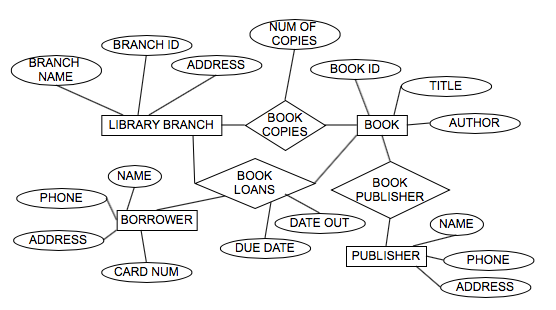
\includegraphics[width=15cm]{images/9-3.png}
\end{center}

Book authors, in this particular diagram, are represented as a multi-valued attribute of books.
\section*{Chapter 11}
\addcontentsline{toc}{section}{Chapter 11}

\subsection*{11.31 Map the COMPANY ER schema in Figure 7.2 into ODL classes. Include appropriate methods for each class.}
\addcontentsline{toc}{subsection}{11.31}

\begin{itemize} \itemsep0em
\item[] \itab{\textbf{class} Employee}
\item[] \itab{( \textbf{extent}} \tab{employees}
\item[] \itab{\hspace{2 mm} \textbf{key}} \tab{ssn} \tab{)}
\item[] \itab{\{ \textbf{attribute}} \tab{\textbf{struct} name} \tab{\{ \textbf{string} fname,}
\item[] \itab{} \tab{} \tab{\hspace{3 mm}\textbf{string} mname,}
\item[] \itab{} \tab{} \tab{\hspace{3 mm}\textbf{string} lname \hspace{2 mm}\} name;}
\item[] \itab{\hspace{2 mm} \textbf{attribute}} \tab{\textbf{string}} \tab{ssn;}
\item[] \itab{\hspace{2 mm} \textbf{attribute}} \tab{\textbf{date}} \tab{bdate;}
\item[] \itab{\hspace{2 mm} \textbf{attribute}} \tab{\textbf{enum}} \tab{Gender{M, F} sex;}
\item[] \itab{\hspace{2 mm} \textbf{attribute}} \tab{\textbf{string}} \tab{address;}
\item[] \itab{\hspace{2 mm} \textbf{attribute}} \tab{\textbf{float}} \tab{salary;}
\item[] \itab{\hspace{2 mm} \textbf{attribute}} \tab{Employee} \tab{supervisor;}
\item[] \itab{\hspace{2 mm} \textbf{relationship}} \tab{Department works\_for \textbf{inverse} Department:: has\_employees;}
\item[] \itab{\hspace{2 mm} \textbf{relationship}} \tab{set<Hours\_Worked> work \textbf{inverse} Hours\_Worked:: work\_by;}
\item[] \itab{\hspace{2 mm} \textbf{short}} \tab{age();}
\item[] \itab{\hspace{2 mm} \textbf{void}} \tab{give\_raise(\textbf{in} \textbf{float} raise);}
\item[] \itab{\hspace{2 mm} \textbf{void}} \tab{change\_address(\textbf{in} \textbf{string} new\_address);}
\item[] \itab{\hspace{2 mm} \textbf{void}} \tab{reassign\_emp(\textbf{in} \textbf{string} new\_dname) \textbf{raises} (dname\_not\_valid); \};}\\
\end{itemize}

\begin{itemize} \itemsep0em
\item[] \itab{\textbf{class} Department}
\item[] \itab{( \textbf{extent}} \tab{departments}
\item[] \itab{\hspace{2 mm} \textbf{key}} \tab{dname, dnumber} \tab{)}
\item[] \itab{\{ \textbf{attribute}} \tab{\textbf{string}} \tab{dname;}
\item[] \itab{\hspace{2 mm} \textbf{attribute}} \tab{\textbf{short}} \tab{dnumber;}
\item[] \itab{\hspace{2 mm} \textbf{attribute}} \tab{\textbf{struct}} \tab{Dept\_Mgr {Employee manager, \textbf{date} startdate} mgr;}
\item[] \itab{\hspace{2 mm} \textbf{attribute}} \tab{set<\textbf{string}>} \tab{locations;}
\item[] \itab{\hspace{2 mm} \textbf{relationship}} \tab{set<Employee> has\_employees \textbf{inverse} Employee:: works\_for;}
\item[] \itab{\hspace{2 mm} \textbf{relationship}} \tab{set<Project> controls \textbf{inverse} Project:: controlled\_by;}
\item[] \itab{\hspace{2 mm} \textbf{short}} \tab{no\_of\_employees();}
\item[] \itab{\hspace{2 mm} \textbf{void}} \tab{add\_emp(\textbf{in} \textbf{string} new\_essn) \textbf{raises} (essn\_not\_valid);}
\item[] \itab{\hspace{2 mm} \textbf{void}} \tab{add\_proj(\textbf{in} \textbf{string} new\_pname) \textbf{raises} (pname\_not\_valid);}
\item[] \itab{\hspace{2 mm} \textbf{void}} \tab{change\_manger(\textbf{in} \textbf{string} new\_mssn; \textbf{in} \textbf{date} startdate) \textbf{raises} (mssn\_not\_valid); \};}\\
\end{itemize}

\begin{itemize} \itemsep0em
\item[] \itab{\textbf{class} Project}
\item[] \itab{( \textbf{extent}} \tab{projects}
\item[] \itab{\hspace{2 mm} \textbf{key}} \tab{pname, pnumber} \tab{)}
\item[] \itab{\{ \textbf{attribute}} \tab{\textbf{string}} \tab{pname;}
\item[] \itab{\hspace{2 mm} \textbf{attribute}} \tab{\textbf{short}} \tab{pnumber;}
\item[] \itab{\hspace{2 mm} \textbf{attribute}} \tab{\textbf{string}} \tab{location;}
\item[] \itab{\hspace{2 mm} \textbf{relationship}} \tab{Department controlled\_by \textbf{inverse} Department:: controls;}
\item[] \itab{\hspace{2 mm} \textbf{relationship}} \tab{set<Hours\_Worked> work\_at \textbf{inverse} Hours\_Worked:: work\_on;}
\item[] \itab{\hspace{2 mm} \textbf{void}} \tab{reassign\_proj(\textbf{in} \textbf{string} new\_dname) \textbf{raises} (dname\_not\_valid) \};}\\
\end{itemize}

\begin{itemize} \itemsep0em
\item[] \itab{\textbf{class} Hours\_Worked}
\item[] \itab{( \textbf{extent}} \tab{hours\_worked )}
\item[] \itab{\{ \textbf{attribute}} \tab{\textbf{float}} \tab{hours;}
\item[] \itab{\hspace{2 mm} \textbf{relationship}} \tab{Employee work\_by \textbf{inverse} Employee:: work;}
\item[] \itab{\hspace{2 mm} \textbf{relationship}} \tab{Project work\_on \textbf{inverse} Project:: work\_at;}
\item[] \itab{\hspace{2 mm} \textbf{void}} \tab{change\_hours(\textbf{in} \textbf{float} new\_hours); \};}\\
\end{itemize}


\begin{itemize} \itemsep0em
\item[] \itab{\textbf{class} Dependent}
\item[] \itab{( \textbf{extent}} \tab{dependents )}
\item[] \itab{\{ \textbf{attribute}} \tab{\textbf{string}} \tab{name;}
\item[] \itab{\hspace{2 mm} \textbf{attribute}} \tab{\textbf{date}} \tab{bdate;}
\item[] \itab{\hspace{2 mm} \textbf{attribute}} \tab{\textbf{enum}} \tab{Gender\{M, F\} sex;}
\item[] \itab{\hspace{2 mm} \textbf{attribute}} \tab{\textbf{string}} \tab{relationship;}
\item[] \itab{\hspace{2 mm} \textbf{attribute}} \tab{Employee} \tab{suporter;}
\item[] \itab{\hspace{2 mm} \textbf{short}} \tab{age(); \hspace{2 mm}\};}\\
\end{itemize}
\section*{Chapter 15}
\addcontentsline{toc}{section}{Chapter 15}

\subsection*{15.21 In what normal form is the LOTS relation schema in Figure 15.12(a) with respect to the restrictive interpretations of normal form that take only the primary key into account? Would it be in the same normal form if the general definitions of normal form were used?}
\addcontentsline{toc}{subsection}{15.21}

By only taking the primary key into account, we can see that the relation schema will be in 2NF since there are no partial dependencies on the primary key. However, our relation schema is not in 3NF due to the fact that the primary key has two transitive dependencies:
\begin{enumerate}
\item[] PROPERTY\_ID$\#$ $\rightarrow$ COUNTY\_NAME $\rightarrow$ TAX\_RATE
\item[] PROPERTY\_ID$\#$ $\rightarrow$ AREA $\rightarrow$ PRICE
\end{enumerate}
By taking all the keys into account, the relation schema will only be in 1NF (just look at the general definitions of 2NF and 3NF). This is because there is a partial dependency on the secondary key {COUNTY\_NAME, LOT\#} listed here:
\begin{enumerate}
\item[]COUNTY\_NAME $\rightarrow$ TAX\_RATE
\end{enumerate}
This violates 2NF.

\subsection*{15.23 Why do spurious tuples occur in the result of joining the EMP\_PROJ1 and EMP\_LOCS relations in Figure 15.5 (result shown in Figure 15.6)?}
\addcontentsline{toc}{subsection}{15.23}

A tuple (e, l) in EMP\_LOCS shows that we have an employee, named e, working on some project at location l. A tuple (s, p, h, pn, l) in EMP\_PROJ1, shows that we have an employee working on project p at location l with social security number s. When these two are joined, the tuple (e, l) can be joined with the tuple (s, p, h, pn, l) where we have e, name of an employee, and s, social security number of a different employee. This results in spurious tuples, leaving us unhappy.

\subsection*{15.27 Consider a relation R(A, B, C, D, E) with the following dependencies:
\begin{center}
AB $\rightarrow$ C, CD $\rightarrow$ E, DE $\rightarrow$ B\\
\end{center}
Is AB a candidate key of this relation? If not, is ABD? Explain your answer.}
\addcontentsline{toc}{subsection}{15.27}

No, AB += \{A,B,C\}, which is a proper subset of \{A,B,C,D,E\}.
Yes, ABD += \{A,B,C,D,E\}.

\subsection*{15.31 Consider the following relation for published books:
\begin{center}
BOOK (Book\_title, Author\_name, Book\_type, List\_price, Author\_affil, Publisher)
\end{center}
Author\_affil refers to the affiliation of author. Suppose the following dependencies exist: Book\_title $\rightarrow$ Publisher, Book\_type Book\_type $\rightarrow$ List\_price Author\_name $\rightarrow$ Author\_affil
\begin{enumerate}
\item What normal form is the relation in? Explain your answer.
\item Apply normalization until you cannot decompose the relations further.
\end{enumerate}
State the reasons behind each decomposition.}
\addcontentsline{toc}{subsection}{15.31}

\begin{enumerate}
\item The key for this relation is Book\_title, Authorname. Since no attributes are FFD on the key, this given relation is in 1NF. It is not in 2NF or 3NF.
\item \begin{enumerate}
\item 2NF decomposition:\\
Book0 (Book\_title, Author\_name)\\
Book1 (Book\_title, Publisher, Book\_type, List\_price)\\
Book2 (Author\_name, Author\_affil)\\
Any partial dependencies are eliminated by this decomposition.
\item 3NF decomposition:\\
Book0 (Book\_title, Author\_name)\\
Book1-1 (Book\_title, Publisher, Book\_type)\\
Book1-2 (Book\_type, List\_price)\\
Book2 (Author\_name, Author\_affil)\\
Luckily, our decomposition eliminates any sort of transitive dependency on Listprice.
\end{enumerate}
\end{enumerate}
\section*{Chapter 16}
\addcontentsline{toc}{section}{Chapter 16}


\subsection*{16.18 Show that, if the matrix $S$ resulting from Algorithm 16.3 does not have a row that is all $a$ symbols, projecting $S$ on the decomposition and joining it back will always produce at least one spurious tuple.}
\addcontentsline{toc}{subsection}{16.18}

For every relation $R$ $i$ in our decomposition, the matrix $S$ initially has one row with $a$ symbols under the columns for the attributes. 
When we project $S$ on each $R$ $i$, the algorithm will produce one row consisting of all $a$ symbols in each S($R$ $i$) since we never change an $a$ symbol into a $b$ symbol during the application of the algorithm. Joining all the $a$ rows in each projection will give us at least one row of all $a$ symbols. So, if $S$ does not have a row that is all $a$, and then we apply this algorithm, our result will have at least one all $a$ row.
This means we have a spurious tuple.

\subsection*{16.19 Show that the relation schemas produced by Algorithm 16.5 are in BCNF.}
\addcontentsline{toc}{subsection}{16.19}
The algorithm loop will only end after all relation schemas are in BCNF.
\section*{Chapter 17}
\addcontentsline{toc}{section}{Chapter 17}

\subsection*{17.27 Consider a disk with the following characteristics (these are not parameters of any particular disk unit): block size B = 512 bytes; interblock gap size G = 128 bytes; number of blocks per track = 20; number of tracks per surface = 400. A disk pack consists of 15 double-sided disks.}
\addcontentsline{toc}{subsection}{17.27}
\subsubsection*{(a) What is the total capacity of a track, and what is its useful capacity (excluding interblock gaps)?}
\begin{description}
\item[Total] 20 * (512 + 128) = 12800 bytes = 12.8 Kbytes
\item[Useful] 20 * 512 = 10240 bytes = 10.24 Kbytes
\end{description}

\subsubsection*{(b) How many cylinders are there?}
\begin{description}
\item[Tracks] $\#$ tracks = $\#$ cylinders = 400
\end{description}

\subsubsection*{(c) What are the total capacity and the useful capacity of a cylinder?}
\begin{description}
\item[Total] 15 * 2 * 20 * (512 + 128) = 384000 bytes = 384 Kbytes
\item[Useful] 15 * 2 * 20 * 512 = 307200 bytes = 307.2 Kbytes
\end{description}

\subsubsection*{(d) What are the total capacity and the useful capacity of a disk pack?}
\begin{description}
\item[Total] 15 * 2 * 400 * 20 * (512 + 128) = 153600000 bytes = 153.6 Mbytes
\item[Useful] 15 * 2 * 400 * 20 * 512 = 122.88 Mbytes
\end{description}

\subsubsection*{(e) Suppose that the disk drive rotates the disk pack at a speed of 2400 rpm (revolutions per minute); what are the transfer rate (TR) in bytes/msec and the block transfer time (BTT) in msec? What is the average rotational delay (RD) in msec? What is the bulk transfer rate? (See Appendix B.)}
\begin{description}
\item[Transfer rate ] TR = (total track size in bytes)/(time for one disk revolution in msec) TR = (12800) / ((60 * 1000) / (2400)) = (12800) / (25) = 512 bytes/msec
\item[Block transfer time] BTT = B / TR = 512 / 512 = 1 msec
\item[Average rotational delay] RD = (time for one disk revolution in msec) / 2 = 25 / 2 = 12.5 msec
\item[Bulk transfer rate] BTR = TR * (B / (B + G)) = 512 * (512/640) = 409.6 bytes/msec
\end{description}

\subsubsection*{(f) Suppose that the average seek time is 30 msec. How much time does it take (on the average) in msec to locate and transfer a single block, given its block address?}
\begin{enumerate}
\item[] S + RD + BTT = 30 + 12.5 + 1 = 43.5 msec
\end{enumerate}

\subsubsection*{(g) Calculate the average time it would take to transfer 20 random blocks, and compare this with the time it would take to transfer 20 consecutive blocks using double buffering to save seek time and rotational delay.}
\begin{description}
\item[Random] 20 * (S + RD + BTT) = 20 * 43.5 = 870 msec
\item[Consecutive] S + RD + 20 * BTT = 30 + 12.5 + (20 * 1) = 62.5 msec
\end{description}

\subsection*{17.37 Can you think of techniques other than an unordered overflow file that can be used to make insertions in an ordered file more efficient?}
\addcontentsline{toc}{subsection}{17.37}
Keeping in mind the manner in which the overflow for static hash files is chained, using an overflow file in which the records are chained together is prudent. Any overflow records inserted in any block of the ordered file are linked together. Just like a linked list, a pointer to the first record in the chain is kept in the block of the main file. The list in our example can be kept ordered or unordered.

\subsection*{17.39 Can you think of techniques other than chaining to handle bucket overflow in external hashing?}
\addcontentsline{toc}{subsection}{17.39}
Internal hashing has many techniwues which can handle bucket overflow. If a bucket is full, the record which should be inserted in that bucket may be placed in the next bucket if there is space, which is reminiscent of a technique called open addressing. Another way of approaching this problem is to simply consider using a whole overflow block for each and every bucket that becomes full.
\section*{Chapter 19}
\addcontentsline{toc}{section}{Chapter 19}


\subsection*{19.17 Can a nondense index be used in the implementation of an aggregate operator? Why or why not?}
\addcontentsline{toc}{subsection}{19.17}
A nondense index contains entries for only some of the search values. A great example of a nondense index is a primary index because it includes an entry for every disk block of a data file as opposed to having one for every record. The nondense index would potentially be able to be used to compute the MIN function. This would be the case if the smallest key value in the data block corresponded to the keys in the index. Due to all the values not appearing in the index, MAX, AVG, SUM and COUNT would not be able to determined.

\subsection*{19.21 Extend the sort-merge join algorithm to implement the LEFT OUTER JOIN operation.}
\addcontentsline{toc}{subsection}{19.21}
Before exteding the sort-merge join algorithmn, let's explain a LEFT OUTER JOIN operation. A LEFT OUTER JOIN of relations $R$ and $S$ would produce all of the rows from $R$ and $S$ that join. It would also produce the rows from $R$ that \textit{do not} join any row from S. In order to extend the sort-merge join algorithm, we only need to modify anything during the merge phase. In the first and second steps of the algorithm, the relations $R$ and $S$ would be soreted on their respective join column or columns. The third step would include them merging of the sorted $R$ and $S$ relations would be merged. If the $R$ row and $S$ row have the same value for the join column, their rows would be combined. Any given $R$ row would also be placed in the LEFT OUTER JOIN result if no matching $S$ row was found. The corresponding attributes from the $S$ relation would simply be NULL values.
\section*{Chapter 22}
\addcontentsline{toc}{section}{Chapter 22}

\subsection*{22.22 Prove that strict two-phase locking guarantees strict schedules.}
\addcontentsline{toc}{subsection}{22.22}
Due to the fact that any transaction that would want to read or write an item being read or written by transaction T must wait until T has committed, a strict schedule is satisfied due to this very condition.
\section*{Chapter 23}
\addcontentsline{toc}{section}{Chapter 23}

\subsection*{23.21 Suppose that the system crashes before the $\lbrack$ read\_item, T3,A $\rbrack$ entry is written to the log in Figure 23.1(b). Will that make any difference in the recovery process?}
\addcontentsline{toc}{subsection}{23.21}

Since read\_item operations are only needed to tell if cascading rollback of supplmentary transactions are necessary, no difference in the recovery process will be seen.

\subsection*{23.22 Suppose that the system crashes before the $\lbrack$ write\_item,T2,D,25,26 $\rbrack$ entry is written to the log in Figure 23.1(b). Will that make any difference in the recovery process?}
\addcontentsline{toc}{subsection}{23.22}

It will. Transactions T2 and T3 would not be commited just yet, so they would have to be rolled back in the recovery process.
\section*{Chapter 24}
\addcontentsline{toc}{section}{Chapter 24}


\subsection*{24.33 Suppose that privilege (a) of Exercise 24.32 is to be given with GRANT OPTION but only so that account A can grant it to at most five accounts, and each of these accounts can propagate the privilege to other accounts but without the GRANT OPTION privilege. What would the horizontal and vertical propagation limits be in this case?}
\addcontentsline{toc}{subsection}{24.33}

A horizontal propagation limit of 5 and a vertical propagation limit of level 1 would be granted to USER\_A. This is so that USER\_A can then grant wothough needing the  GRANT OPTION. USER\_A would have a level 0 vertical limit allowing him or her to grant it to at most five other users. After this, USER\_A cannot further grant any more privileges.
\section*{Chapter 26}
\addcontentsline{toc}{section}{Chapter 26}


\subsection*{26.37 Consider the UNIVERSITY EER schema in Figure 8.10. Write some rules (in English) that could be implemented via active rules to enforce some common integrity constraints that you think are relevant to this application.}
\addcontentsline{toc}{subsection}{26.37}

\begin{enumerate}
	\item Whemever any student, graduate or undergraduate, withdraws from a class notify their teacher.
	\item If a student receives transcripts from other schools and has classes for credit form that institution, notify their advisor if their class standing changes.
	\item If a student graduates, add them to the alumni mailing list and notify alumni relations.
	\item If a student assistant is eventually hired as a full time employee, raise her or his salary 10\%.
\end{enumerate}




% \section*{Chapter 28}
\addcontentsline{toc}{section}{Chapter 28}


\subsection*{28.15 Show two rules that have a confidence of 0.7 or greater for an itemset containing three items from Exercise 28.14.}
\addcontentsline{toc}{subsection}{28.15}

We can see that there really is only one itemset with a size of 3: \{$milk, bread, eggs$\}. For our first rule, we can try rule $milk, eggs$ $\rightarrow$ $bread$. The confidence of this rule exceeeds the minumum confidence value of 0.7 since it is is $0.3/0.3$. For our second rule, let's try $bread$ $\rightarrow$ $milk, eggs$. The confidence of this rule satisfies the min confidence requirement since it is $0.3/0.4$.


\end{document}  